\section{Block Diagram}

The block diagram of  mmRISC-1 is shown in Figure \ref{fig:BLOCKDIAGRAM}. The mmRISC-1 contains multiple CPU Harts and a Debug Module with JTAG/cJTAG interface. Each Hart has an instruction fetch bus, a data access bus, and a monitor bus for LR/SC operation. The Debug Module has a dedicated system bus access capability and controls each Hart (run / stop / step, etc.). The Debug Module can access resources in each Hart such as programmer’s model registers (XRn, FRn), SCR (System Control Registers) and memory-mapped devices through data access bus by debugger’s abstract commands.\\
Each Hart consists of an instruction fetch unit with a pre-fetch buffer, a pipeline unit with an instruction decoder, a datapath unit for integer operations, CSR resources, debugger support, and a floating point operation unit. The monitor bus for LR/SC operation exists only when the Atomic ISA is enabled. The floating point operation unit exists only when the floating-point ISA is enabled.\\

\begin{figure}[H]
    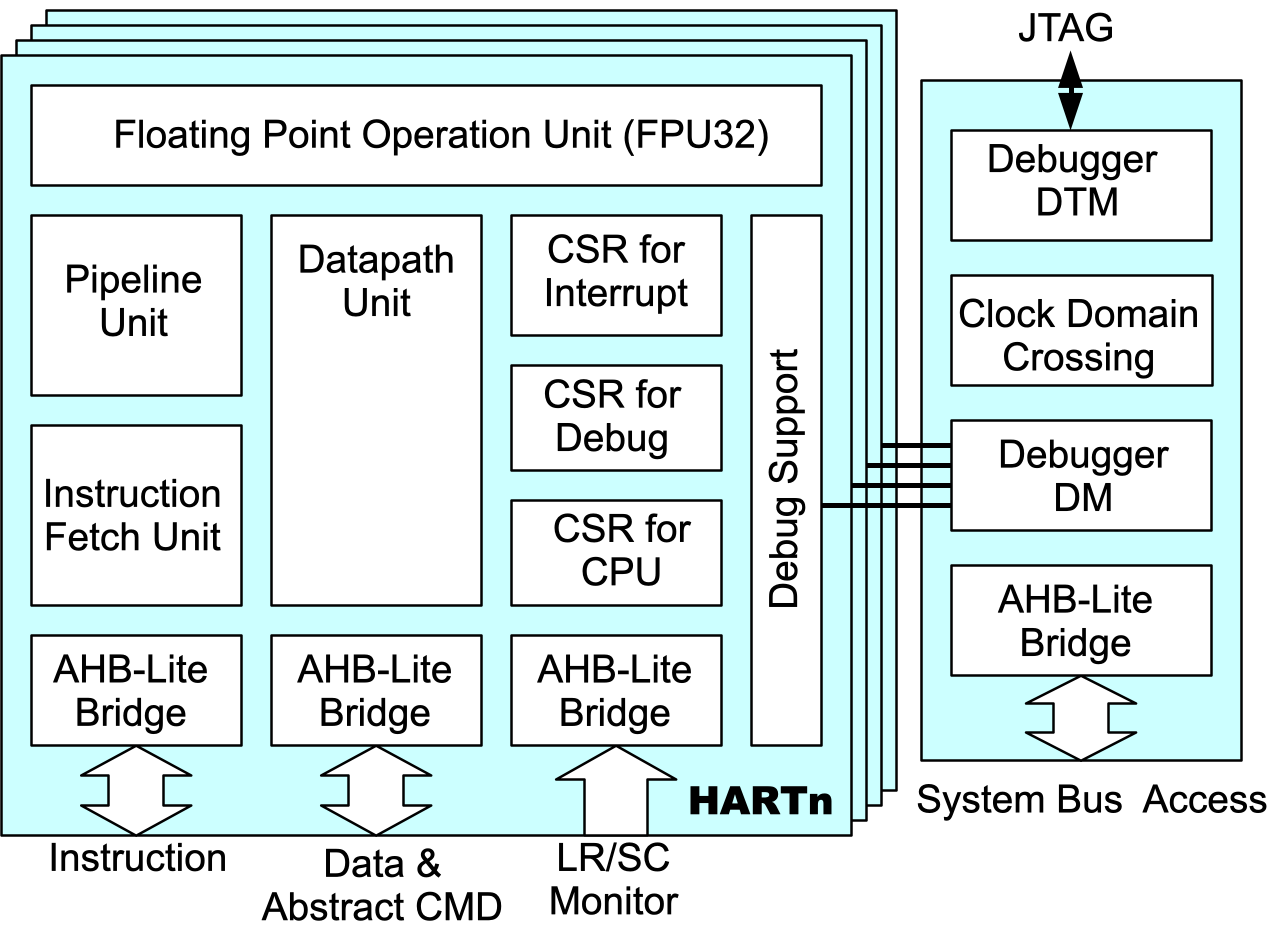
\includegraphics[width=1.00\columnwidth]{./Figure/BlockDiagram.png}
    \caption{mmRISC-1 Block Diagram\protect\footnotemark[1]}
    \label{fig:BLOCKDIAGRAM}
\end{figure}
\footnotetext[1]{cJTAG is supported by logics at outside of mmRISC core.}
